\documentclass[tikz,border=10pt]{standalone}
\usepackage{amsmath}
\usepackage{tikz}
\usetikzlibrary{arrows.meta, positioning}

\begin{document}
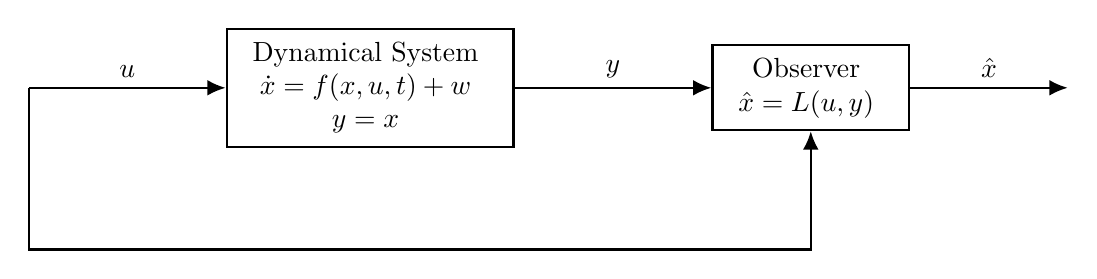
\begin{tikzpicture}[
    block/.style = {draw, thick, minimum height=3em, minimum width=6em, align=center},
    arrow/.style = {thick, -{Latex[width=2mm]}},
    node distance=2.5cm and 2.5cm
  ]

  % System block
  \node[block] (system) {
    \begin{tabular}{c}
      Dynamical System \\
      $\dot{x} = f(x,u,t) + w$ \\
      $y = x$
    \end{tabular}
  };

  % Observer block to the right
  \node[block, right=of system] (observer) {
    \begin{tabular}{c}
      Observer \\
      $\hat{x} = L(u, y)$ 
    \end{tabular}
  };

  % u input line with elbow to system and to observer from below
  \coordinate[left=2.5cm of system] (input);
  \coordinate[below=1.5cm of observer] (belowobserver);

  \draw[arrow] (input) -- node[above] {$u$} (system.west);
  \draw[arrow] (input) |- (belowobserver) -| (observer.south);

  % y from system to observer (midpoints)
  \draw[arrow] (system.east) -- node[above] {$y$} (observer.west);

  % Output x̂ from observer
  \draw[arrow] (observer.east) --++ (2cm, 0) node[midway, above] {$\hat{x}$};

\end{tikzpicture}
\end{document}
